\documentclass{beamer}

\input{../ts-glærur}

\title{FOR3R - Röðunarreiknirit III}

\begin{document}
\begin{frame}
\titlepage
\end{frame}

\section{Counting Sort}

\begin{frame}{Counting Sort}

\begin{itemize}
 \item Counting sort er röðunarreiknirit nokkuð ólíkt þeim sem við höfum kynnst
 \item Byggir ekki á samanburðum
  \begin{itemize}
  \item Stöðugt
  \item Erfitt að fastákveða tímaflækju - línulegt fall af inntaksstærð, en það segir hér ekki alla söguna
  \item Minnisþörf einnig a.m.k. línulegt fall af inntaksstærð
  \end{itemize}
\end{itemize}
\end{frame}

\begin{frame}{Um Counting Sort}
\begin{itemize}
 \item Eins og nafnið bendir til byggist Counting Sort á \emph{talningu}
 \item Gerir ráð fyrir heiltölum á bilinu $0 \ldots k$ sem inntaki
 \begin{enumerate}
  \item Fyrst er búið til aukafylki af stærð $k$
  \item Fjöldi staka af hverri tölu á bilinu $0 \ldots k$ er talin og geymd í aukafylkinu
  \item Summað er yfir fylkið svo aukafylkið innihaldi fjölda staka sem eru minni en vísirinn í upphaflega fylkinu
  \item Annað aukafylki er búið til og raðað inn í það eftir fjöldanum.
 \end{enumerate}
\end{itemize}
\end{frame}

\begin{frame}[fragile]{Counting Sort - sauðakóði}
\begin{center}
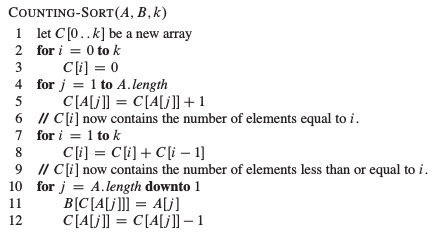
\includegraphics[scale=0.8]{Pics/counting-sort-pseudocode}
\end{center}
\end{frame}

\begin{frame}{Hluti af ferlinu}
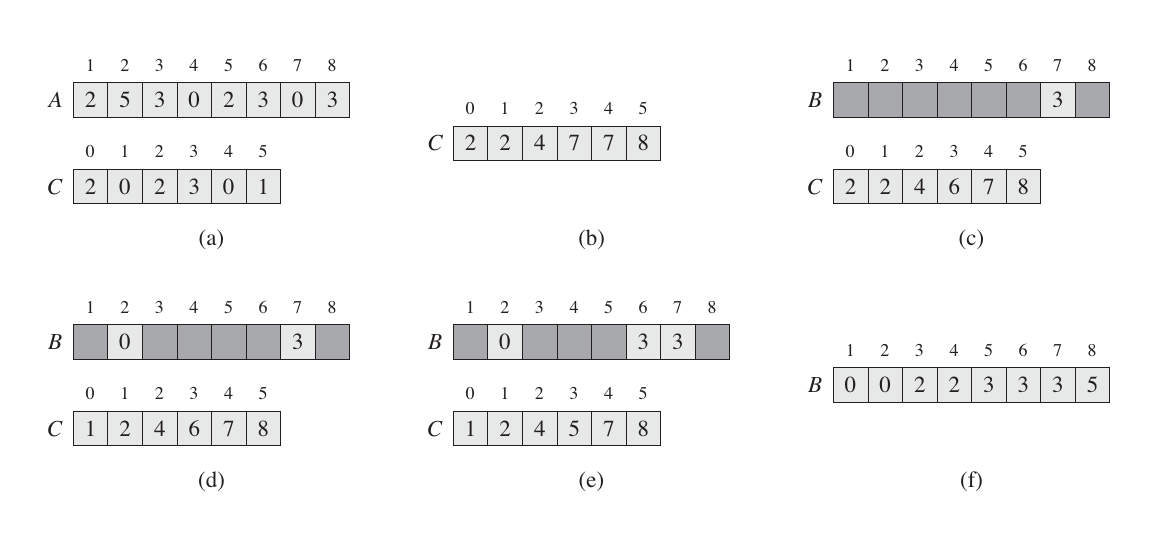
\includegraphics[width=\textwidth]{Pics/CountingSort}
\end{frame}

\section{Radix Sort}

\begin{frame}{Radix sort}
\begin{itemize}
 \item Counting sort virkar illa þegar bil talnanna er breitt.
 \item Hægt er að skipta röðunarvandamáli fyrir stórar heiltölur upp
 \begin{itemize}
  \item Einum ``staf'' raðað í einu
 \end{itemize}
 \item Slík útfærsla er kölluð \emph{radix sort}
 \begin{itemize}
  \item T.d. ``decimal radix''
 \end{itemize}
\end{itemize}
\end{frame}

\begin{frame}[fragile]{(LSD) Radix sort - sauðakóði}
Gerum ráð fyrir að hver tala í listanum $A$ hafi $d$ stafi. Þá er hægt að raða listanum með eftirfarandi aðferð:
\begin{verbatim}
radix_sort(A,d)
  for i = to d
    use a stable sort to sort array A on digit i
\end{verbatim}
Hér er stöðuga röðunarreikniritið oft counting sort.
\end{frame}

\begin{frame}{Hluti af ferlinu}
Hér er \emph{least significant digit} útfærsla á radix sort sýnd:
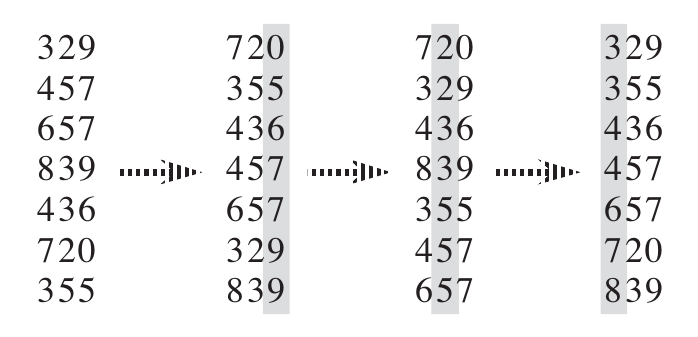
\includegraphics[width=\textwidth]{Pics/RadixSort}
\end{frame}

\begin{frame}{LSD vs. MSD}
\begin{itemize}
 \item Hægt er að byrja röðunina á minnst markverða tölustafnum (e. \emph{least significant digit}, LSD) eða mest markverða tölustafnum (e. \emph{most significant digit}, MSD)
 \item MSD:
 \begin{itemize}
  \item Skiptir listanum niður í ``fötur'' sem hægt er að raða endurkvæmt
  \item Þarfnast aukageymslu til að vera stöðugt
 \end{itemize}
 \item LSD:
 \begin{itemize}
  \item Einfaldara (sjá sauðakóða)
  \item Stöðugt
 \end{itemize}
\end{itemize}
\end{frame}

\begin{frame}{Tímaflækja Radix sort}
\begin{itemize}
 \item Það að nota Radix sort til að raða $n$ staka lista af tölum af lengd $d$ þar sem hvert sæti getur tekið $k$ mismunandi gildi tekur $O(d(n+k))$ tíma.
 \begin{itemize}
  \item Ýmsar framsetningar á þessu ($d$ eða $k$ hunsað)
 \end{itemize}
 \item MSD er almennt hraðvirkara í raunverulegum útfærslum
\end{itemize}

\end{frame}


\begin{frame}{YouTube}
\begin{itemize}
 \item \href{https://www.youtube.com/watch?v=LyRWppObda4}{Radix sort - LSD}
 \item \href{https://www.youtube.com/watch?v=Tmq1UkL7xeU}{Radix sort - MSD}
\end{itemize}
\end{frame}

\begin{frame}{Frekari lesning}
\begin{itemize}
 \item Counting sort: Kafli 8.2
 \item Radix sort: Kafli 8.3
\end{itemize}

\end{frame}


\end{document}
